%%GM
%%Grey model 灰色预测

\subsection{GM}

\subsubsection{GM(1,1)}

%%设系统主变量原始数据序列为
\begin{displaymath}
X^{(0)}=(x^{(0)}(1),x^{(0)}(2),\ldots,x^{(0)}(m))
\end{displaymath}
%%其依次累加生成(Accumulating Generate Operator)序列为
\begin{displaymath}
X^{(1)}=(x^{(1)}(1),x^{(1)}(2),\ldots,x^{(1)}(m))
\end{displaymath}
%%其中
\begin{displaymath}
x^{(1)}(i)=\sum_{j=1}^{i}{x^{(0)}(j)}
\end{displaymath}
%%而序列
\begin{displaymath}
Z^{(1)}=(-,z^{(1)}(2),z^{(1)}(3),\ldots,z^{(1)}(m))
\end{displaymath}
%%被称为$X^{(1)}$的均值生成序列或系统的背景值，其中
\begin{displaymath}
z^{(1)}(i)=\frac{1}{2}(x^{(1)}(i)+x^{(1)}(i-1)),\qquad i=2,3,\ldots,m
\end{displaymath}
%%则称方程
\begin{displaymath}
x^{(0)}(i)+az^{(1)}(i)=b
\end{displaymath}
%%为一阶单变量灰色预测模型(One Order Single Variable Grey Model, $GM(1,1)$模型)。其中参数$a$是主变量参数或系统发展系数，$b$是$GM(1,1)$模型的灰作用系数或背景值。$\hat{a}=(a,b)^{T}$通过最小二乘方法取得，即设
\begin{displaymath}
Y=\left[
\begin{matrix}
x^{(0)}(2)\\
x^{(0)}(3)\\
\vdots\\
x^{(0)}(m)\\
\end{matrix}
\right]
\end{displaymath}

\begin{displaymath}
B=\left[
\begin{matrix}
-z^{(1)}(2) & 1 \\
-z^{(1)}(3) & 1 \\
\vdots & \vdots \\
-z^{(1)}(m) & 1 \\
\end{matrix}
\right]
\end{displaymath}
%%则
\begin{displaymath}
\hat{a}=(B^TB)^{-1}B^TY
\end{displaymath}
%%方程
\begin{displaymath}
\frac{\dif x^{(1)}}{\dif t}+ax^{(1)}=b
\end{displaymath}
%%被称为$GM(1,1)$模型的白化方程，也叫影子方程。结合$\hat{a}=(B^TB)^{-1}B^TY$所求解的$a,b$参数值，代入$\frac{dx^{(1)}}{dt}+ax^{(1)}=b$，可得$GM(1,1)$模型的时间响应序列为
\begin{displaymath}
\hat{x}^{(1)}(k+1)=(x^{(0)}(1)-\frac{b}{a})e^{-ak}+\frac{b}{a},\qquad k=2,3,\cdots,m-1
\end{displaymath}
%%通过上式可以求解依次累加生成序列$X^{(1)}$的模拟值$\hat{X}^{(1)}$，
\begin{displaymath}
\hat{X}^{(1)}=(\hat{x}^{(1)}(1),\hat{x}^{(1)}(2),\cdots,\hat{x}^{(1)}(m))
\end{displaymath}
%%运用方程
\begin{displaymath}
\hat{x}^{(0)}(k+1)=\hat{x}^{(1)}(k+1)-\hat{x}^{(1)}(k)
\end{displaymath}
%%可分别求解原始序列的模拟值和预测值$\hat{x}^{(0)}(k)$，排列所有$\hat{x}^{(0)}(k)$值可得原始序列的模拟值序列
\begin{displaymath}
\hat{X}^{(0)}=(\hat{x}^{(0)}(1),\hat{x}^{(0)}(2),\ldots,\hat{x}^{(0)}(m))
\end{displaymath}
%%结合$X^{(0)}=(x^{(0)}(1),x^{(0)}(2),\ldots,x^{(0)}(m))$和$\hat{X}^{(0)}=(\hat{x}^{(0)}(1),\hat{x}^{(0)}(2),\cdots,\hat{x}^{(0)}(m))$计算平均绝对误差(Mean Absolute Percent Error, MAPE)可得出模型仿真效果，MAPE被定义为
\begin{displaymath}
MAPE(\%)=\frac{1}{n}\sum_{k=1}^{n}|\frac{x^{(0)}(k)-\hat{x}^{(0)}(k)}{x^{(0)}(k)}|
\end{displaymath}
\par
%%对应上文所述灰色预测模型构建的一般分析过程，$GM(1,1)$模型的构建原理如下。\par
%%通常来说，如果输出数据$x^{(0)}(k)$适用于$GM(1,1)$，那么可以用MAPE来分析原始数据序列$X^{(0)}(k)$和模拟数据序列$\hat{X}^{(0)}(k)$之间的误差。事实上，$GM(1,1)$模型之所以是一个特殊灰色预测模型，只有主变量序列被考虑在模型的构建过程中，而不考虑任何其他影响因素。因此，$GM(1,1)$模型通常被用来研究系统主变量的自回归演化。从输入信息和输出结果来看，$GM(1,1)$模型的建模过程与其他时变预测模型相似。模拟序列的数据随着时间的变化而变化。不同的是，$GM(1,1)$模型构建是基于累加生成数据而其他时变预测模型基于原始序列。建模过程中，原始数据的随机扰动经过累加生成过程被大大减弱，使得系统增长规律得以涌现，即使当数据较少时，$GM(1,1)$模型仍然能够取得较好的模拟和预测效果。

\begin{figure}[H]
    \centering
    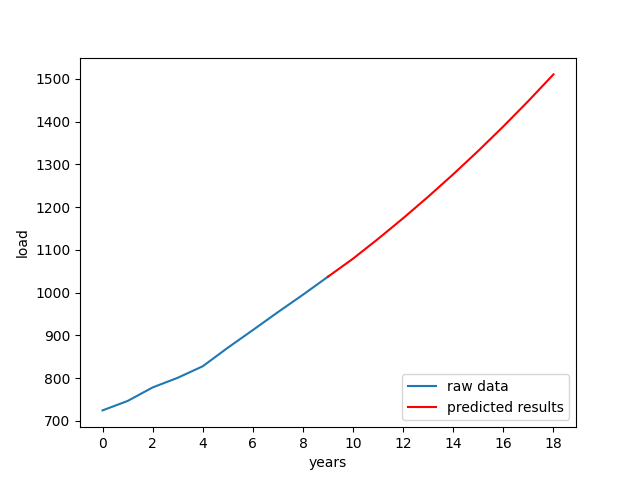
\includegraphics[width=\linewidth]{Models/prediction/GM/GM.png}
    \caption{prediction result}
    \label{fig:prediction result}
\end{figure}